\addsection{Heroes}{\images/sorcery.png}
\hypertarget{Heroes}{Players} always control a Main Hero and may additionally also recruit a Secondary Hero.
A “player’s Hero” may refer to either of them.
Heroes are used to perform Movement Actions on the game board and to start Combats against enemies in order to reach a Scenario victory condition.

\subsection*{Main Hero}
The Main Hero is represented by its chosen model and Hero Card.
Each Faction’s Main Hero has 3 Movement Points.
Only the Main Hero can use your deck.\par
Each Main Hero starts the game at Level 1 and can advance up to Level 7 by gaining Experience.
Experience is gained from \hyperlink{Combatexperience}{winning Combat}, Visiting certain \hyperlink{All}{Locations} and the \hyperlink{Resources}{Treasure Die} \includesvg[height=10px]{\svgs/trasuredie.svg}.
Gaining 1 Experience is represented by the symbol \includesvg[height=10px]{\svgs/exp.svg}.

\subsection*{\hypertarget{Secondary}{Secondary Heroes}}
If you control a Town or a Settlement, a Secondary Hero can be Hired by flipping your \textbf{Population Token} and paying 10 Gold \includesvg[height=10px]{\svgs/gold.svg}.
\textbf{Note}: Units \textbf{cannot} be \hyperlink{Units}{recruited or reinforced} during that use of the Population Token.\par
Your Secondary Hero uses the remaining Hero model of your Faction.
You may wish to mark this model with a token such as a Faction Cube to differentiate it from the Main Hero.
After Hiring a Secondary Hero, place the model in a Town or Settlement you control.
\textbf{You can only have one Secondary Hero at a time}.\par
Secondary Heroes have 2 Movement Points; when you gain one, take an additional set of 2 Movement Tokens to represent their MP.
They do not have their own Hero Card, cannot gain Experience, and cannot use cards from Your Deck for any reason.
If a Secondary Hero gains any cards, \hyperlink{Playerdecks}{place them into your hand} as normal.
Secondary Heroes are considered to have the same Level as the Main Hero for the purposes of resolving \hyperlink{Quick}{Quick Combat}.\par
If your Secondary Hero is attacked by an enemy Hero, you can choose to have your Hero be \hyperlink{Endcombat}{instantly defeated instead of fighting a Combat}.
When a Secondary Hero is defeated, remove them from the game.
They can be recruited again with another use of the Population Token.\par

\clearpage

\subsection*{\hypertarget{Herocard}{Hero Card Anatomy}}
\bigbreak
\begin{figure}[h]
  \begin{minipage}[t]{0.5\textwidth}
    \vspace{0pt}
    \begin{enumerate}[itemsep=5pt]
      \item \textbf{Name} – The Hero’s name.
        Used for identification.
        Has no gameplay effect.
      \item \textbf{Class} – The Hero’s class.
        Has no gameplay effect.
      \item \textbf{Type} – The Hero’s type (Might \includesvg[height=10px]{\svgs/might.svg} or Magic \includesvg[height=10px]{\svgs/magic.svg}).
        Determines the amount of Magic Arrow Spells in your Starting Deck (1 or 2 respectively).
      \item \textbf{Faction Color} – Reminder for the color of the Faction’s cubes and miniatures.
      \item \textbf{Attack} – Number of Attack cards in your Starting Deck.
      \item \textbf{Defense} – Number of Defense cards in your Starting Deck.
      \item \textbf{Power} – Number of Power cards in your Starting Deck.
      \item \textbf{Knowledge} – Number of Knowledge cards in your Starting Deck.
      \item \textbf{Starting Ability} – Reminder for the unique Ability card the Hero starts with.
      \item \textbf{Hero Specialty} – Reminder for the Specialty cards the Hero adds to their deck at the start of the game and after specific Level ups.
        Each hero has three Specialty Cards.
      \item \textbf{Level Tracker} – Whenever a Main Hero gains 1 or more Experience \includesvg[height=10px]{\svgs/exp.svg}, move the cube that number of steps on this track.
        When the cube reaches the next slot on the upper row, the hero gains a Level.
    \end{enumerate}
  \end{minipage}\hfill
  \begin{minipage}[t]{0.48\textwidth}
    \centering
    \vspace{0pt}
    \begin{scriptsize}
      \begin{tikzpicture}
        \draw (0, 0) node[inner sep=0] {\makebox[\textwidth][c]{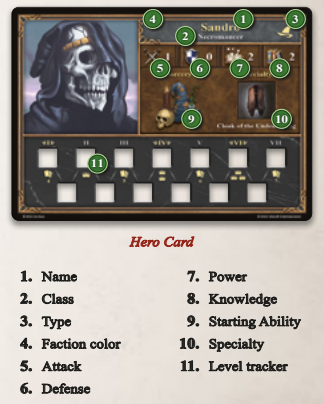
\includegraphics[width=\linewidth]{\images/herocard.png}}};
        \draw (2.2, 2.5) node {\encircle{\phantom{.}1\phantom{.}}};
        \draw (0.8, 1.9) node {\encircle{\phantom{.}2\phantom{.}}};
        \draw (3.5, 2.5) node {\encircle{\phantom{.}3\phantom{.}}};
        \draw (-0.1, 2.5) node {\encircle{\phantom{.}4\phantom{.}}};
        \draw (0, 1.25) node {\encircle{\phantom{.}5\phantom{.}}};
        \draw (1.1, 1.25) node {\encircle{\phantom{.}6\phantom{.}}};
        \draw (2, 1.25) node {\encircle{\phantom{.}7\phantom{.}}};
        \draw (3.25, 1.25) node {\encircle{\phantom{.}8\phantom{.}}};
        \draw (1, -0.2) node {\encircle{\phantom{.}9\phantom{.}}};
        \draw (3, -0.2) node {\encircle{10}};
        \draw (-1.7, -1.4) node {\encircle{11}};
      \end{tikzpicture}
    \end{scriptsize}
    \break
    \footnotesize{\textbf{\textit{\textcolor{darkcandyapplered}{Hero Card}}}}
    \scriptsize
    \begin{multicols}{2}
      \begin{itemize}
        \item[\textbf{1.}] \textbf{Name}
        \item[\textbf{2.}] \textbf{Class}
        \item[\textbf{3.}] \textbf{Type}
        \item[\textbf{4.}] \textbf{Faction Color}
        \item[\textbf{5.}] \textbf{Attack}
        \item[\textbf{6.}] \textbf{Defense}
        \item[\textbf{7.}] \textbf{Power}
        \item[\textbf{8.}] \textbf{Knowledge}
        \item[\textbf{9.}] \textbf{Starting Ability}
        \item[\textbf{10.}] \textbf{Specialty}
        \item[\textbf{11.}] \textbf{Level Tracker}
        \item[\textbf{\phantom{.}}] \phantom{.}
      \end{itemize}
    \end{multicols}
  \end{minipage}
\end{figure}

\clearpage

\subsection*{\hypertarget{Level}{Level Effects}}
Main Heroes always start each Scenario at Level 1 and may Level up by gaining Experience \includesvg[height=10px]{\svgs/exp.svg}.
The most common sources of gaining Experience are the \hyperlink{Resources}{Treasure Die} and \hyperlink{Combatexperience}{Combat}.
Each new Level up requires \textbf{2 Experience}.
When a Main Hero reaches a new Level, resolve the effects of the Level up immediately.
Gaining Experience at Level 7 has no effect.\par
The Level Tracker on your hero card shows the following information:
\begin{itemize}
\item Your Main Hero’s current Level and amount of Experience gained, shown by the cube's position.
\item Your current Hand Limit \includesvg[height=10px]{\svgs/hand.svg}.
\item The number of \hyperlink{Ability}{Expert Effects} \includesvg[height=10px]{\svgs/expert.svg} you may use during a round.
\item At which Levels your main hero must \hyperlink{Playerdecks}{\textbf{Search}} for a new \hyperlink{Ability}{Ability Card} or gain a \hyperlink{Specialty}{Specialty Card}.
Level numbers written in gold on the level tracker (\includesvg[height=10px]{\svgs/level1.svg}, \includesvg[height=10px]{\svgs/level4.svg} and \includesvg[height=10px]{\svgs/level6.svg}) give you a Specialty Card, while silver levels (2, 3, 5, 7) give you an Ability Card.
\end{itemize}
List of all effects:
\begin{itemize}
\item \textbf{Level 1} – Your Hand Limit is 4.
Add your first Specialty Card to Your Deck.
\item \textbf{Level 2} – Search (2) the Ability Deck.
You may play 1 card for their Expert Effect per round.
\item \textbf{Level 3} – Your Hand Limit is 5.
Search (2) the Ability Deck.
\item \textbf{Level 4} – Gain your second Specialty Card.
You may play 2 cards for their Expert Effect per round.
\item \textbf{Level 5} – Your Hand Limit is 6.
Search (2) the Ability Deck.
\item \textbf{Level 6} – Gain your third Specialty Card.
You may play 3 cards for their Expert Effect per round.
\item \textbf{Level 7} – Your Hand Limit is 7.
Search (2) the Ability Deck.
\end{itemize}
